\documentclass{article}
\usepackage{glossaries}
\usepackage{graphicx}

\graphicspath{/Images}

\makeglossaries

\newglossaryentry{map}
{
    name = map,
    description = {The playable area in which the player can move around and interact
    with}
}

\newglossaryentry{dialog}
{
    name = {dialog system},
    description = {The system in which dialog is shown to the player to talk to the player}
}

\newglossaryentry{egg}
{
    name = {easter egg},
    description = {A hidden non-essential secret for the players to discover}
}

\newglossaryentry{interact}
{
    name = interact,
    description = {The player can interact with the environment by opening doors,
    picking up a key and taking damage from tiles.}    
}

\newglossaryentry{FOW}
{
    name = {Fog Of War},
    description = {A system in which the player can only see what is immediately around
    them and what they have previously explored.}    
}

\newglossaryentry{DialogObjects}
{
    name = {dialog obejcts},
    description = {A scriptable object in which the dialog text,position,colour, identification,duration
    and next dialog ID is stored}
}

\newglossaryentry{ScriptOBJ}
{
    name = {scriptable obejct},
    description = {A unity class which stores data}
}

\newglossaryentry{WS}
{
    name = {world space},
    description = {The in game space}
}

\newglossaryentry{GO}
{
    name = {game object},
    description = {Objects within the game}
}

\newglossaryentry{RT}
{
    name = {render texture},
    description = {A unity texture that can update during runtime}
}

\newglossaryentry{Magic}
{
    name = {magic circle},
    description = {the boundary that divides ideas and
    activities that are meaningful in the game from those that are meaningful in
    the real world} 
}



\begin{document}



\section{General description}
The prototype will be a 2D top down game in which the player will be given the task
of escaping the \gls{map} that they were put in.

\begin{figure}[ht!]
    \centering
    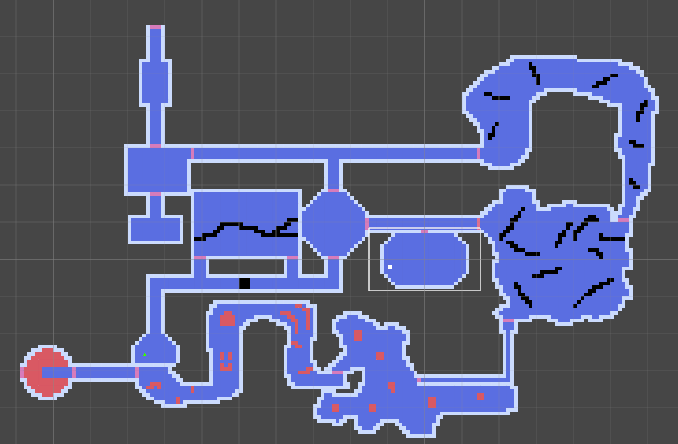
\includegraphics[width=0.4\textwidth]{Images/FinishedMap.png}
    \caption{The map that the player can explore}
    \label{img:FinishedMap}
\end{figure}



\section{Mechanics}
The player is able to move and \gls{interact} with the environment, the main 
\gls{interact}s will be picking up an object to escape and getting damaged
by the environment.



\subsection{Actions and Challenges}
The challenge of the game is exploration in which the player needs to explore the \gls{map}
in order to escape from the \gls{map}.
The player will be able to move around in a 2D \gls{map} and \gls{interact} with an object
within that \gls{map}. 
The player may face the challenge of if they should listen to the \gls{dialog} or not
along with moving around hazards on the \gls{map}.



\begin{figure}[ht!]
    \centering
    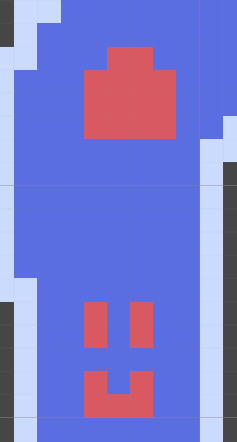
\includegraphics[width=0.4\textwidth, height=0.4\textwidth]{Images/MapHazards.png}
    \caption{Hazards the player must avoid}
    \label{img:MapHazards}
\end{figure}



Another challenge the player faces is remembering where they are and where they went when
navigating the \gls{map}.
The player speed was set to a speed in which the player can easily move around the \gls{map}
while still having time to read the dialog given by the \gls{dialog}.
The player has to dodge hazards on the \gls{map} mainly red tiles which damage the player every 2
seconds the player is touching the tile. If the player takes more than 3 damage within
5 seconds the player dies. This system allows the player to make mistakes and recover from
them by waiting before they move on.




\subsection{Genre}
The genre of the game would be a Narrative game. This genre is seen when the player
is guided through dialog to what they should do. The \gls{dialog} also tells the 
player a story which the player can piece together by trying to get all the dialog.
\newline
Some sub-genres include: Horror. The horror element comes from the game limiting
the player's vision in order to hide information from the player.



\subsection{Game examples}
\subsubsection*{The Stanley Parable: Different endings and narrator}
In The Stanley Parable the player is guided through the game by a narrator who tells
the player what the player should do. The player can decide to listen to the narrator
or go against the narrator. Different endings can be achieved based off of if the 
player listened to the narrator or not.
The \gls{dialog} in the prototype will work similar to the narrator in Stanley Parable
where the system will guide the player to a specific outcome and the player can decide
if they want to listen or not. Unlike in The Stanley Parable the \gls{dialog} will not
remember what the player did the previous playthrough.
\subsubsection*{DarkWood: Fog Of War}
The \gls{FOW} in DarkWood only allows the player to see the general shape of the \gls{map}
while showing the player only a small area around them along with where the character is 
looking. The \gls{FOW} system will work similar to the one in DarkWood but the player
will only be allowed to see what is around their character not just where their character
is looking.


\newpage
\section{Interrogation}

\subsection{Hypothesis}
The player will explore other aspects of the game that they have not found if
they know there is more to find even when a clear winning goal is shown.



\subsection{Goals}
\begin{itemize}
    \item To spark the player's curiosity through a \gls{dialog} that will speak to the
    player. The \gls{dialog} can either say words that help the player or hinder them.
    \item To limit the player's vision through either a \gls{FOW} system or a field of view system
    in order to get the player curios about what they cannot see and get the player to explore
    more of the \gls{map}. 
\end{itemize}




\newpage
\section{Process}
User input code has been used from a previous project. The code uses a \gls{ScriptOBJ}
to read the user inputs while the scripts that use these inputs subscribe to events from
the \gls{ScriptOBJ} to use them.
Item pooling code was used from a previous project for the dialog.
A generic tilemap was made in Asseprite to use for a \gls{map}.
\newline
Different ways \gls{FOW} was tried:
\newline
To make the \gls{FOW} a tutorial page was followed online mainly form Success Knocks[1]
where the steps where outlined in how to make the \gls{FOW}. A youtube tutorial[2] was
followed in order to code the shaders needed for the \gls{FOW}.
\newline
A \gls{RT} was used along with shaders 
that paint the texture white. Two different shaders were used the \gls{FOW}
and vision. The \gls{FOW} shader is a completely black shader that then checks for
if there is any vision material and will then change the \gls{RT} to white in
the area that the material is allowing the player to see that area. The reason that
this solution did not work was the uv's between the \gls{FOW} camera and the Main camera
where not aligning, which can be seen in Figure \ref{img:FOWflawed}, which caused the vision 
circle to be stretched.
\newline
A solution to this problem was disabling the global light from unity and putting a 
spot light around the player as seen in Figure \ref{img:LightSolution}.
\newline
The \gls{dialog} was decided to be in world space instead of an overlay of the 
camera to make it that the player can miss dialog due to them not waiting for the
dialog to finish. Dialog objects where made in order to store the data needed for the \gls{dialog}.
This data would then be read by a manager script which creates dialog in the
game. 
\newline
The \gls{map} is rigid in places where the \gls{dialog} wants the player to be while 
the \gls{map} turns flexible where the player should not be according to the \gls{dialog}.



\begin{figure}[ht!]
    \centering
    \begin{minipage}[b]{0.4\textwidth}
        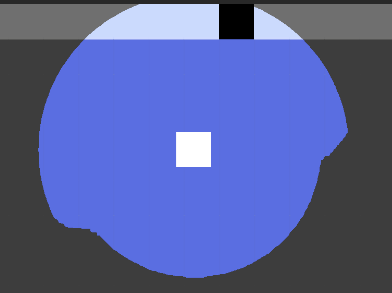
\includegraphics[width=\textwidth]{Images/StreachedFOW.png}
        \caption{Image of flawed Fog Of War}
        \label{img:FOWflawed}
    \end{minipage}
    \hfill
    \begin{minipage}[b]{0.4\textwidth}
            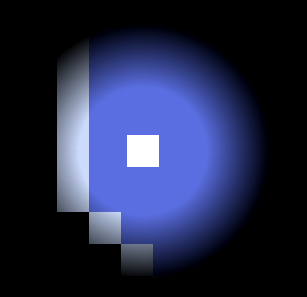
\includegraphics[width=\textwidth]{Images/LightSolution.png}
            \caption{Image of light solution}
            \label{img:LightSolution}
    \end{minipage}
\end{figure}




\section{Reflection}
During the prototype I successfully coded the \gls{dialog}. This was done using
dialog objects which stored the data of the dialog, dialog game objects which held 
the dialog objects and the dialog manager which used all the dialog scriptable objects
in order to make the dialog in the \gls{WS}. This system solidified how important file 
management is due to the amount of dialog objects that were made during the assignment.
During the first few days of the project I was working on the Fog Of War system which 
led me to learning about hlsl unity which stands for high level shader language. This
coding language is used by unity for its shaders. I started learning this language
through the youtube video [2]. This was a time consuming process which caused me to 
stop working on the system after 4 days due to needing to work on the other parts of the 
assignment, thus the light solution was used due to time constraints. 
This assignment helped me solidify my coding fundamentals to code for general situations where
the code can be reused in different contexts along. This will help me in the future because
I can reuse the code done in this assignment for other assignments which will make the future
assignments easier. 
\newline
Through play testing it was found that the players did not trust 
the dialog system until they explored more of the \gls{map} which helped prove the 
hypothesis made that players will explore when they know they can even when a 
clear goal is shown.





\section{Player motivation design}
To motivate the player extrinsically the \gls{dialog} was made which gives the player a clear guide
and goal where the goal is to escape the \gls{map}. The \gls{dialog} can also just talk to the player
without giving them a clear way to go.
\newline
The game also breaks the \gls{Magic} [3] by telling the player to exit back to main menu
in one of the endings. Along with this magic circle break the player is given a hint 
about how to get another ending.
The player's actions may also change depending on what the \gls{dialog} tells them,
for example if the \gls{dialog} tells the player to go left the player may just be
motivated to go right.
\newline
To keep the player intrinsically motivated they need to be made curios about the game. This will
be achieved by the \gls{dialog} telling them that there is still something more to do even after the 
player achieved an ending, which leads the player to play the game again in order to find
what they missed. 
\newline
If the \gls{dialog} is fleshed out and does dialog based
on what the player does in the game then the player will try new actions in order to
see what the \gls{dialog} will tell them.
\newline
An \gls{egg} was placed in the game for the player to discover. This helps in getting
the player to explore more of the \gls{map}.



\section{References}
[1]“Success Knocks | The Business Magazine,” Success Knocks | The Business Magazine, Dec. 03, 2025. https://successknocks.com/implementing-dynamic-fog-of-war-in-unity-for-rts/ (accessed Mar. 10, 2026)
\newline
[2]Daniel Ilett, “Your First Shader | Unity Shader Code Basics 01,” YouTube, Oct. 06, 2025. https://www.youtube.com/watch?v=eMWrMRdP5jY (accessed Mar. 10, 2026).
\newline
[3]E. Adams, Fundamentals of game design, 3rd ed. Berkeley, Ca: New Riders, 2014.


\glsaddall
\printglossary

\end{document}